\chapter{Evaluation}
\label{ch:evaluation}
This chapter will cover the execution and evaluation of our benchmark with the workloads specified in section~\ref{ch:design:se:workloads}.
In section~\ref{ch:evaluation:se:overview} we will show which workloads we will compare with each other.
We will present the results of each workload and have a discussion on them directly after that.

A conclusion will be drawn in section~\ref{ch:futureWork:se:conclusion} of the next chapter.

\section{Objective}
The main goal is to find out,
whether databases are capable of handling production workloads.
Besides that,
we will investigate whether we can generalise graph database benchmark results by comparing our results with the results of other studies examining the performance of graph databases with social network graphs.
The generalisation would allow for a performance evaluation of graph databases in an industrial environment with the results from benchmarks performed with social network graphs.

We will measure the average time per operation.
With that we can calculate the throughput in $ \frac{operations}{s} $,
which we will use to compare the different databases.

\section{Setup}
In this section we will describe the software and hardware we used to execute the benchmark.

\subsection{Hardware}
The machine we used for the benchmark was configured as shown in table~\ref{tab:hardware}.

\begin{table}[!h]
  \begin{minipage}{\textwidth}
    \begin{tabularx}{\textwidth}{ | l | X | }
      \hline
      Component & Description \\ \hline \hline
      CPU & Intel i7-3770K @ 3.5GHz \\ \hline
      RAM & 16GB DDR3 @ 1.600MHz \\ \hline
      Storage & Seagate ST2000DL003 2 TB 5900rpm, only a 400GB partition was used \\ \hline
      GPU & NVIDIA GeForce GTX 670 \\ \hline
    \end{tabularx}
  \end{minipage}
  \caption{The hardware specifications of the machine used for the benchmark.}
  \label{tab:hardware}
\end{table}

\subsection{Software}
The versions of the software components we used are shown in table~\ref{tab:software}.

\begin{table}[!h]
  \begin{minipage}{\textwidth}
    \begin{tabularx}{\textwidth}{ | X | X | }
      \hline
      Software & Version \\ \hline \hline
      Ubuntu & 17.10 \\ \hline
      Java & 1.8.0\_171 \\ \hline
      OpenSSH & 7.5p1 \\ \hline
      YCSB & 0.14.0-SNAPSHOT \\ \hline
      Apache Jena & 3.6.0 \\ \hline
      Neo4j & 3.3.4 \\ \hline
      OrientDB & 2.2.33 \\ \hline
      Sparksee & 5.2.3 \\ \hline
    \end{tabularx}
  \end{minipage}
  \caption{The software specifications of the machine used for the benchmark.}
  \label{tab:software}
\end{table}

\section{Overview}
\label{ch:evaluation:se:overview}
In figure~\ref{fig:executionWorkflow} the execution process is illustrated and explained with the following enumeration.

\begin{enumerate}[label=Step \arabic*:,widest=Step 1,leftmargin=*]
  \item One \textbf{workload} is chosen from the set of workloads.
  \item The \textbf{dataset} is \textbf{created} for that workload.
  \item One \textbf{database} is chosen from the set of databases.
  \item The workload is \textbf{executed} on the database with the created dataset.
  \item The \textbf{results} of the benchmark run are stored in a folder specific to the constellation of workload,
  database and execution pass.
  \item Repeat from Step 4 three times.
  \item Repeat from Step 3 until all databases ware benchmarked.
  \item Repeat from Step 1 until all workloads have been executed.
\end{enumerate}

\begin{figure}[!h]
  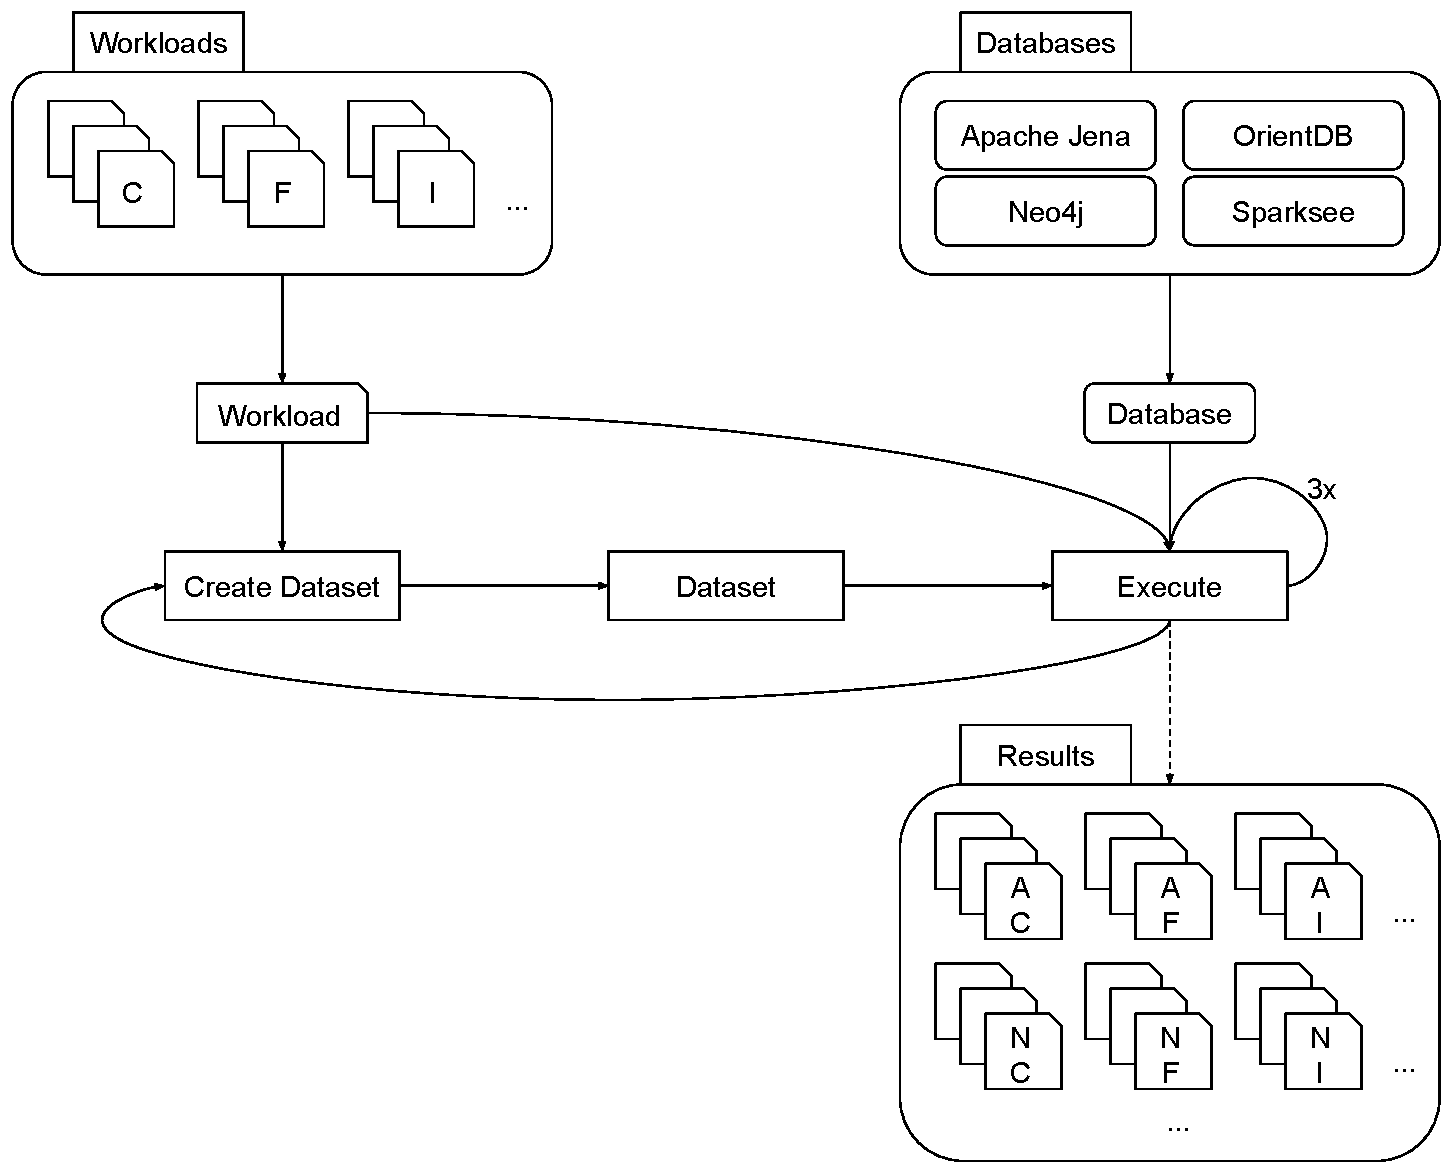
\includegraphics[width=\textwidth]{images/executionWorkflow}
  \caption{Workflow for the execution process.}
  \label{fig:executionWorkflow}
\end{figure}

In table~\ref{tab:throughputOverview} and~\ref{tab:productionOverview} the groups of workloads we are comparing with each other are shown.
The naming of the workloads is similar to the naming introduced in section~\ref{ch:design:se:workloads}.

\begin{table}
  \begin{minipage}{\textwidth}
    \centering
    \begin{tabularx}{\textwidth}{ | l | l | l | X | }
      \hline
      Section & First workload & Other workload(s) & Units of measurement \\ \hline
      \ref{ch:evaluation:se:probingNodeCount} & 1. With Index & 2.-5. With Index & Inserts/second, total time \\ \hline
      \ref{ch:evaluation:se:probingNodeCount} & 1. Without Index & 2.-5. Without Index & Inserts/second \\ \hline
      \ref{ch:evaluation:se:probingNodeCount} & n.\footnote{the workload with the largest possible number of nodes in terms of execution time} With Index & n. Without Index & Inserts/second \\ \hline
      \ref{ch:evaluation:se:probingNodeSize} & 1. Node Size & 2.-5. Node Size & Inserts/second, database size \\ \hline
      \ref{ch:evaluation:se:differenceEdges} & n. With Index & 1. No Edges & Inserts/second \\ \hline
    \end{tabularx}
  \end{minipage}
  \caption{Overview for the throughput workloads.}
  \label{tab:throughputOverview}
\end{table}
\begin{table}
  \begin{minipage}{\textwidth}
    \centering
    \begin{tabularx}{\textwidth}{ | l | l | X | X | }
      \hline
      Section & First workload & Other workload(s) & Units of measurement \\ \hline
      \ref{ch:evaluation:se:productComplexity} & 1. Structure & 2.-3. Structure & Inserts/second \\ \hline
      \ref{ch:evaluation:se:productionSuitability} & x.\footnote{every workload will be evaluated} Suitability & - & Total time \\ \hline
      \ref{ch:evaluation:se:retrievingUnderLoad} & 1. Reading & 2. Reading & Reads/second \\ \hline
      \ref{ch:evaluation:se:retrievingUnderLoad} & 1. Scanning & 2. Scanning & Scans/second \\ \hline
      \ref{ch:evaluation:se:retrievingUnderLoad} & 1. Structure & 1. Reading \& 1. Scanning & Operations/second \\ \hline
    \end{tabularx}
  \end{minipage}
  \caption{Overview for the production and retrieval workloads.}
  \label{tab:productionOverview}
\end{table}

After execution we have to combine the results from the various folders for further examination.
Figure~\ref{fig:evaluationWorkflow} illustrates this process of evaluation.
With all the results in one place we filter the measurements for those we want and calculate the average over the three benchmark runs.
Next,
we group the measurements as shown in tables~\ref{tab:throughputOverview} and~\ref{tab:productionOverview}.\\

\begin{figure}[!h]
  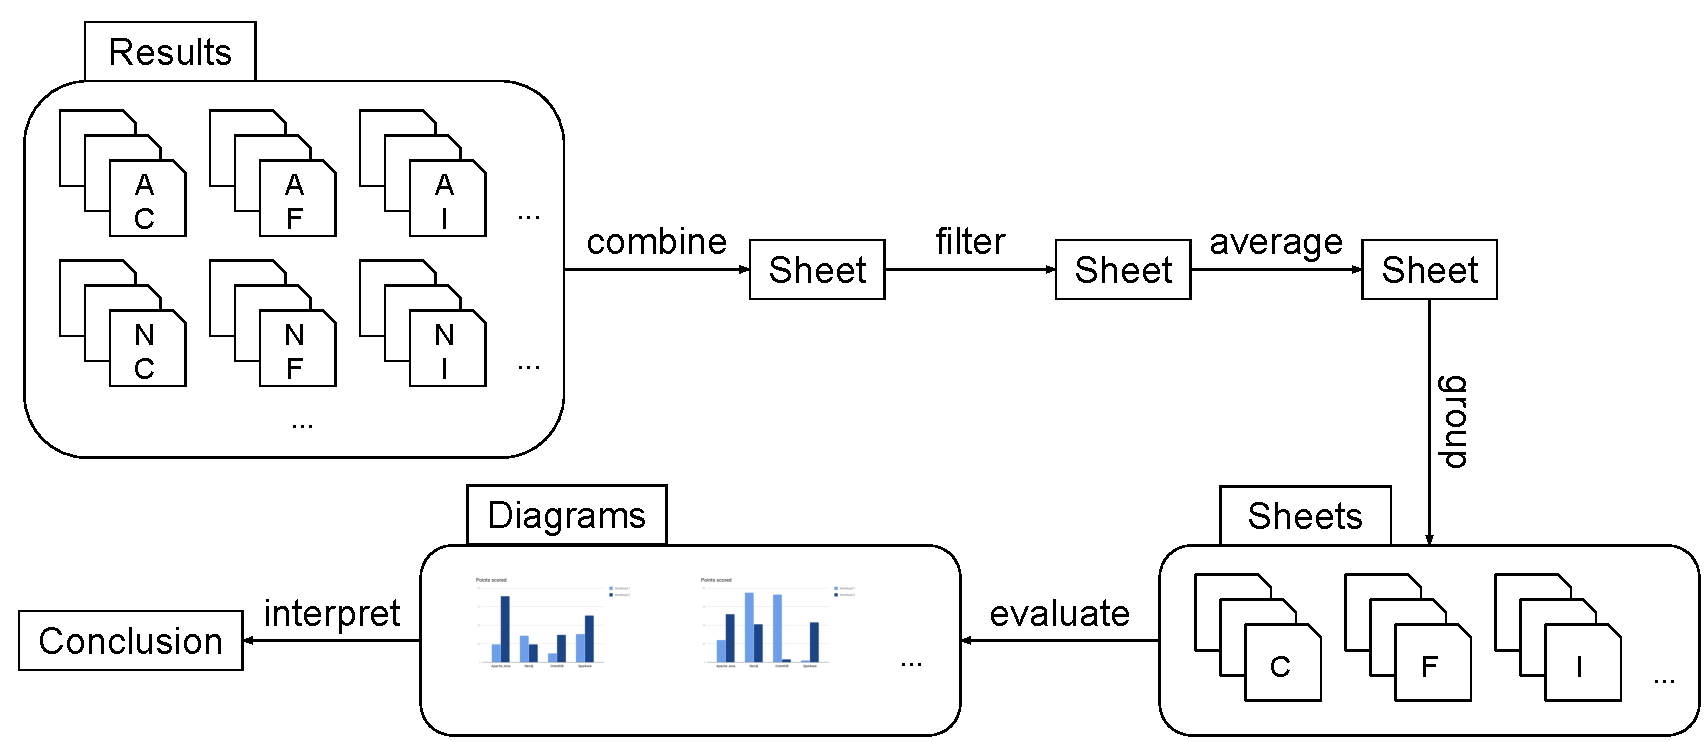
\includegraphics[width=\textwidth]{images/evaluationProcess}
  \caption{Workflow of the evaluation process.}
  \label{fig:evaluationWorkflow}
\end{figure}

Finally,
we create the diagrams shown in the "Results" subsections and interpret them to draw a conclusion in the "Discussion" subsections of the following sections.
The standard derivation isn't shown in the diagrams,
as it is around 5\% for OrientDB and below 1\% for the other databases,
which is too small to be seen in the figures.

\section{Throughput}
\label{ch:evaluation:se:throughput}
In this section we will examine the combinations of workloads mentioned in table~\ref{tab:throughputOverview}.
The throughput will show us how well suited the graph databases are in general for applications heavily using insert operations.

Note that in order to insert an edge the start and end node have to be looked up.

\subsection{Probing Node Count}
\label{ch:evaluation:se:probingNodeCount}
Here we will compare how the throughput,
of the databases changes when increasing the number of nodes we are inserting into it.
We will also look at the execution time,
to determine a reasonable large dataset in terms of execution time for the upcoming benchmark runs.

The throughput is listed in inserts per seconds,
which includes both inserting nodes and inserting edges.

Apache Jena has no option to turn off indexing as mentioned in section~\ref{ch:background:se:apacheJena},
but it is still shown in the diagrams as reference.

\subsubsection{Results}
The first figure~\ref{fig:withIndexThroughput} shows how the different databases perform with an increasing dataset size.
Apache Jena and Neo4j only have values for 1000 and 10000 nodes,
because execution with more than 10000 nodes would take too much time.
Sparksee only delivered results up to 100000 nodes,
because the free license only included database sizes with up to 1000000 elements and a workload with 1000000 nodes would contain 2333333 elements in total.

In figure~\ref{fig:withIndexExecutionTime} we see the execution time of the different databases.
At 10000 nodes Apache Jena and Neo4j took almost an hour for one run,
because of that we didn't run it with 100000 nodes or more.

Tables~\ref{tab:withIndexThroughput},
\ref{tab:withIndexExecutionTime} and~\ref{tab:withoutIndexThroughput} show the measured numbers from figures~\ref{fig:withIndexThroughput},
\ref{fig:withIndexExecutionTime} and~\ref{fig:withoutIndexThroughput} respectively.

\begin{table}[h!]
  \begin{minipage}{\textwidth}
    \centering
    \begin{tabularx}{\textwidth}{ | l | X | X | X | X | X | }
      \hline
      Database/\# Nodes & 1000 & 10000 & 100000 & 1000000 & 10000000 \\ \hline
      Apache Jena & 8,86 & 7,21 & T & T & T \\ \hline
      Neo4j & 11,50 & 8,75 & T & T & T \\ \hline
      OrientDB & 884,1 & 2317,07 & 5672,69 & 10112,36 & 8572,34 \\ \hline
      Sparksee & 15109,17 & 17829,1 & 16425 & L & L \\ \hline
    \end{tabularx}
  \end{minipage}
  \caption{Throughput in inserts/s, rounded to two decimal places, of the workload using an index for the different dataset sizes. T indicates that too much time would be needed; L indicates license issues.}
  \label{tab:withIndexThroughput}
\end{table}

\begin{table}[h!]
  \begin{minipage}{\textwidth}
    \centering
    \begin{tabularx}{\textwidth}{ | l | X | X | X | X | X | }
      \hline
      Database/Time (s) & 1000 & 10000 & 100000 & 1000000 & 10000000 \\ \hline
      Apache Jena & 263 & 3238 & T & T & T \\ \hline
      Neo4j & 203 & 2667 & T & T & T \\ \hline
      OrientDB & 3,64 & 10 & 41 & 231 & 2722 \\ \hline
      Sparksee & 0,15 & 1,31 & 14 & L & L \\ \hline
    \end{tabularx}
  \end{minipage}
  \caption{Execution time in seconds of the workload using an index for the different dataset sizes. T indicates that too much time would be needed; L indicates license issues.}
  \label{tab:withIndexExecutionTime}
\end{table}

\begin{table}[h!]
  \begin{minipage}{\textwidth}
    \centering
    \begin{tabularx}{\textwidth}{ | l | X | X | X | X | X | }
      \hline
      Database/\# Nodes & 1000 & 10000 & 100000 & 1000000 & 10000000 \\ \hline
      Apache Jena & 8,79 & 7,41 & T & T & T \\ \hline
      Neo4j & 12,3 & 8,83 & T & T & T \\ \hline
      OrientDB & 1020,81 & 2357,49 & 4616,85 & 9395,86 & 8415,18 \\ \hline
      Sparksee & 4715,63 & 635,17 & 63,37 & L & L \\ \hline
    \end{tabularx}
  \end{minipage}
  \caption{Throughput in inserts/s, rounded to two decimal places, of the workload using no index for the different dataset sizes. T indicates that too much time would be needed; L indicates license issues.}
  \label{tab:withoutIndexThroughput}
\end{table}

\begin{figure}[h!]
  \centering
  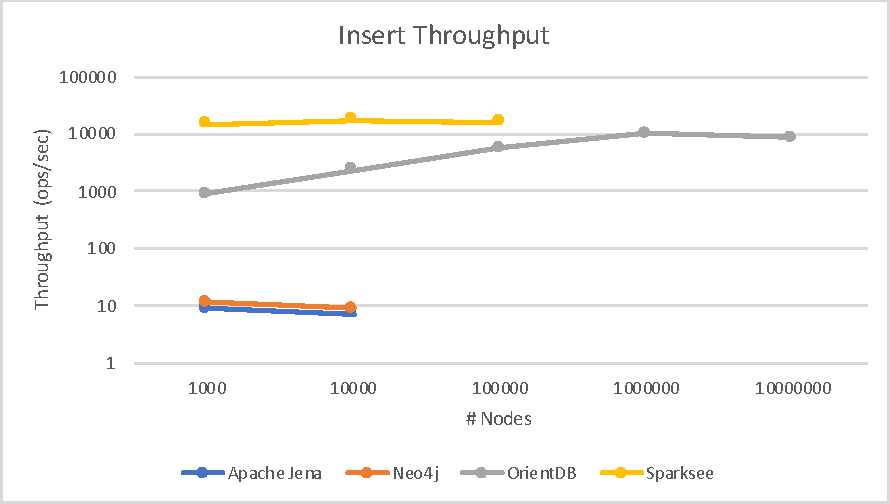
\includegraphics[width=.75\textwidth]{images/throughput/withIndexThroughput}
  \caption{This figure shows the throughput in inserts/second of every database over different dataset sizes.}
  \label{fig:withIndexThroughput}
\end{figure}

\begin{figure}[h!]
  \centering
  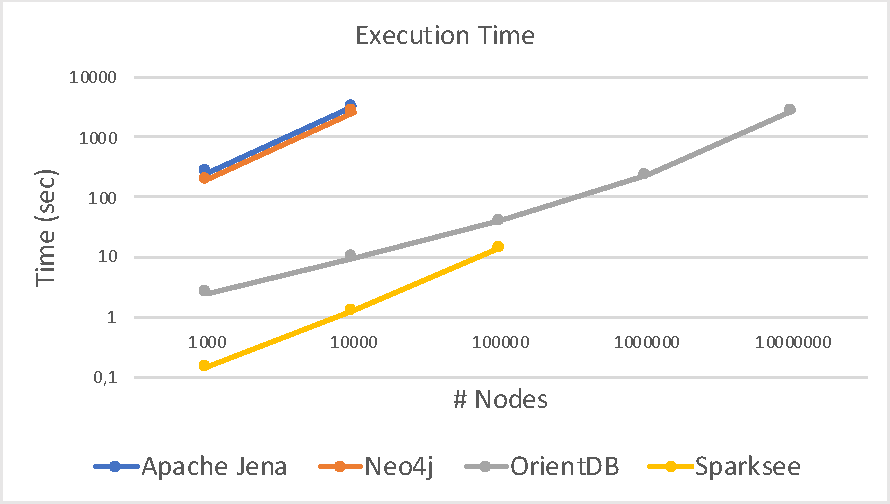
\includegraphics[width=.75\textwidth]{images/throughput/withIndexExecutionTime}
  \caption{The execution time of the databases is shown over different dataset sizes.}
  \label{fig:withIndexExecutionTime}
\end{figure}

Figure~\ref{fig:withoutIndexThroughput} shows the throughput over different dataset sizes without using an index.
In figure~\ref{fig:withWithoutIndexThroughputFixNodes} we see a comparison of using an index and not with a dataset size of 10000 nodes.

\begin{figure}[h!]
  \centering
  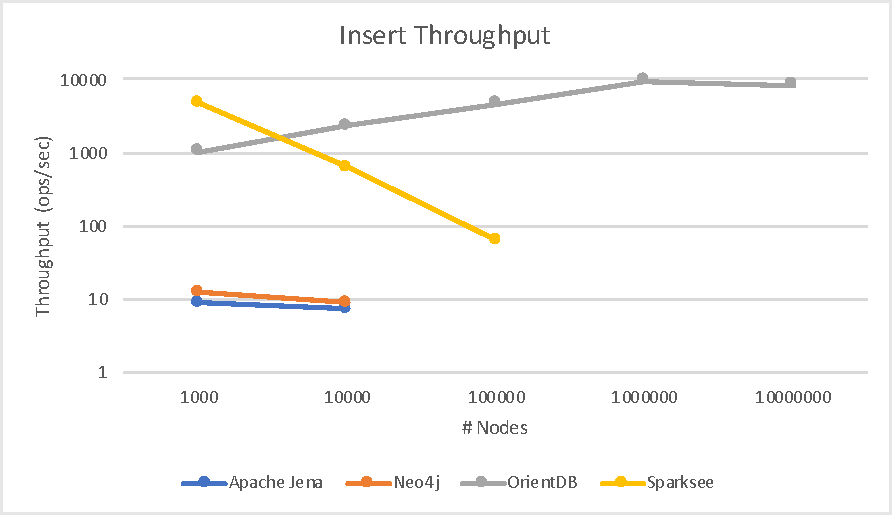
\includegraphics[width=.75\textwidth]{images/throughput/withoutIndexThroughput}
  \caption{This diagram shows the throughput in inserts per second while using no index.}
  \label{fig:withoutIndexThroughput}
\end{figure}

\begin{figure}[h!]
  \centering
  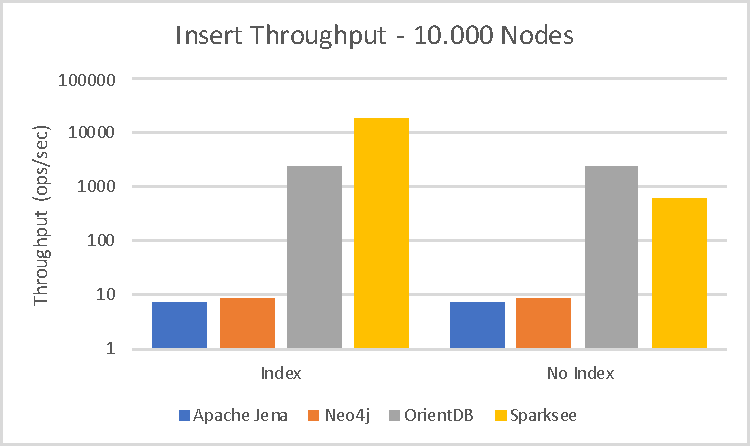
\includegraphics[width=.75\textwidth]{images/throughput/withWithoutIndexThroughputFixNodes}
  \caption{The throughput at a fixed dataset size to compare between indexing and not.}
  \label{fig:withWithoutIndexThroughputFixNodes}
\end{figure}

\subsubsection{Discussion}
Figure~\ref{fig:withWithoutIndexThroughputFixNodes} shows us,
that there is no performance change for Jena, Neo4j and OrientDB in using an index or not.
Sparksee shows a significant drop in throughput without the use of an index.
That is what we expected,
because the throughput also contains insertions of edges,
for which nodes have to be looked up,
which is faster with an index.
For the other databases the lack of difference in performance might be,
because the benefit of using an index to retrieve the nodes for an edge is equalised by the time it takes to insert the nodes into the index.

The throughput is quite stable for most databases,
except OrientDB which grows in throughput until 1000000 nodes and keeps stable for larger datasets.
That means,
that the performance of the databases does scale for larger datasets.

If we compare the archived throughput with our target throughput of $ 11743,66 \frac{inserts}{s} $,
we see that Sparksee exceeds our target with $ 16435 \frac{inserts}{s} $.
OrientDB misses our goal slightly,
it only archived a throughput of $ 8572 \frac{inserts}{s} $ with the largest dataset.
Jena and Neo4j didn't even reach $ 100 \frac{inserts}{s} $.
These throughput values are measured with another data structure and node size than the one we will use for the suitability workload.
We will investigate the factors differentiating this workload from the suitability workload and reference these results again in section~\ref{ch:evaluation:se:suitabilityDiscussion}.

From these results alone,
without looking at read performance separately we can say,
that an index is useful,
even for insert operations,
because to insert an edge two nodes need to be looked up,
which is faster if an index is used.

\subsection{Probing Node Size}
\label{ch:evaluation:se:probingNodeSize}
In this subsection we will take a look at how the databases perform with different node property sizes.
We will pick a dataset size of 10000 nodes,
as all database have a reasonable execution time with that number of nodes.

By investigating the performance under node size variation,
we will see whether the databases can store large numbers of data in each node.
That can be useful depending on the use case,
in our example given by the industry only a two-digit number is stored,
but it could be desirable to store longer numbers or more complex information.

\subsubsection{Results}
In figure~\ref{fig:nodeSize} we see,
how an increasing node size has an impact on insert throughput.

Sparksee only has values for node sizes up to $ 1KB $,
because the property we used to store the value of the node only supports up to 2048 characters or Bytes.

Figure~\ref{fig:sizeDatabaseSize} shows the size of the database folder,
in which the database stores its files.

Tables~\ref{tab:nodeSize} and~\ref{tab:sizeDatabaseSize} show the numbers used for the figures~\ref{fig:nodeSize} and~\ref{fig:sizeDatabaseSize} respectively.

\begin{table}[h!]
  \begin{minipage}{\textwidth}
    \centering
    \begin{tabularx}{\textwidth}{ | X | l | l | l | l | l | l | }
      \hline
      Node Size (Byte)/Database & 10 & 100 & 1000 & 10000 & 100000 & 1000000 \\ \hline
      Apache Jena & 7,21 & 9,66 & 7,83 & 7,54 & 6,21 & 4,92 \\ \hline
      Neo4j & 8,75 & 11,47 & 8,31 & 8,59 & 8,17 & 4,06 \\ \hline
      OrientDB & 2317,07 & 2521,90 & 3141,73 & 1976,84 & 487,21 & 14,10 \\ \hline
      Sparksee & 17829,10 & 17155,63 & 15670,67 & x & x & x \\ \hline
    \end{tabularx}
  \end{minipage}
  \caption{Throughput in inserts/s, rounded to two decimal places, of the workload using different node sizes. x indicates issues when storing large values.}
  \label{tab:nodeSize}
\end{table}

\begin{table}[h!]
  \begin{minipage}{\textwidth}
    \centering
    \begin{tabular}{ | l | l | l | l | l | l | l | }
      \hline
      Node Size (Byte)/Database & 10 & 100 & 1000 & 10000 & 100000 & 1000000 \\ \hline
      Apache Jena & 15 & 16 & 25 & 113 & 994 & 9600 \\ \hline
      Neo4j & 24 & 29 & 49 & 244 & 2200 & 22000 \\ \hline
      OrientDB & 75 & 77 & 98 & 172 & 1300 & 9500 \\ \hline
      Sparksee & 4,7 & 6 & 15 & x & x & x \\ \hline
    \end{tabular}
  \end{minipage}
  \caption{Database sizes of the workload using different node sizes. x indicates issues when storing large values.}
  \label{tab:sizeDatabaseSize}
\end{table}

\begin{figure}[h!]
  \centering
  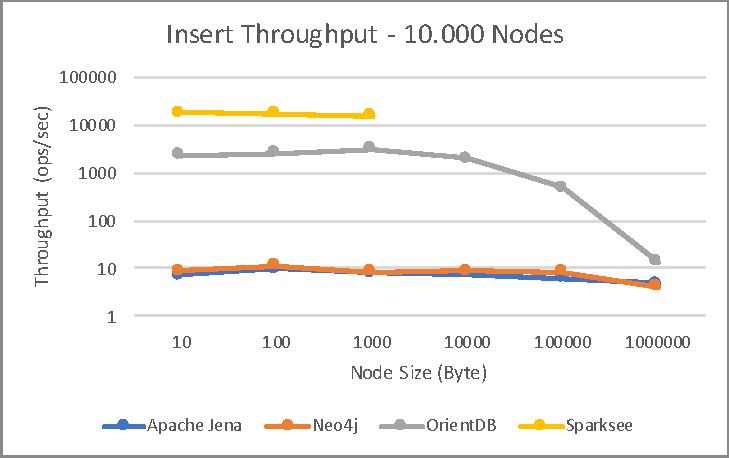
\includegraphics[width=.75\textwidth]{images/throughput/nodeSize}
  \caption{Insert throughput over different node sizes with 10000 nodes total.}
  \label{fig:nodeSize}
\end{figure}

\begin{figure}[h!]
  \centering
  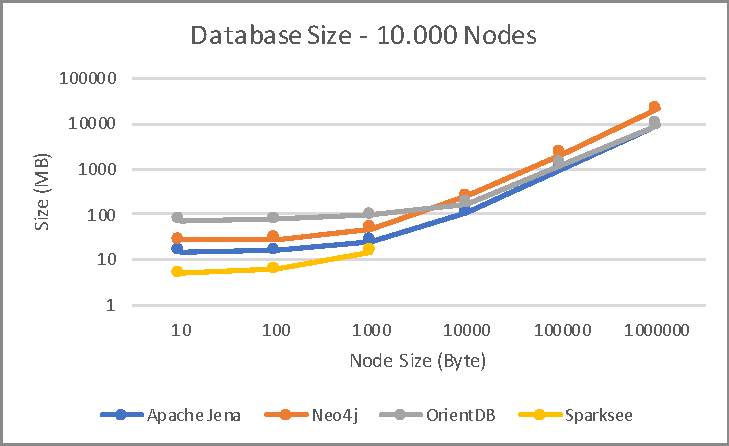
\includegraphics[width=.75\textwidth]{images/throughput/sizeDatabaseSize}
  \caption{The size of the database folders over growing node sizes with 10000 nodes total.}
  \label{fig:sizeDatabaseSize}
\end{figure}

\subsubsection{Discussion}
Figure~\ref{fig:nodeSize} shows that the throughput of Jena and Neo4j is quite low and it doesn't show much difference with larger node sizes,
but at $ 1MB $ we can see that the performance decreases even more.

For OrientDB we see good performance up to $ 1KB $.
It starts to decline for node sizes of $ 10KB $ and above with a significant drop in throughput at $ 1MB $.

Sparksee has the highest throughput of all four databases,
but it could only handle sized of up to $ 2KB $ or $ 1KB $ in our test scenario.
In that range the other databases also show no noteworthy change in performance,
so we can't draw a conclusion about the behaviour of Sparksee with larger node sizes.

In figure~\ref{fig:sizeDatabaseSize} we see that the database size grows linearly with the node size,
from $ 10KB $ and above.
For smaller node values the overhead of the database itself determines the size of the database.

When we look closely at the values of Neo4j,
we can see that they are above the other databases.
In fact,
at $ 1MB $ node size,
which would result in $ 10GB $ data for 10000 nodes,
Neo4js database folder had a size of $ 22GB $,
so the overhead is more than the data itself.

\subsection{Difference without Edges}
\label{ch:evaluation:se:differenceEdges}
In this subsection we will investigate how the absence of edges impacts performance.
These workloads do not represent a real-world scenario,
but they will provide us knowledge about how the e/n ratio effects throughput,
as for every edge its start and end node have to be looked up.

\subsubsection{Results}
Table~\ref{tab:indexNoEdges10000Nodes} and figure~\ref{fig:indexNoEdges10000Nodes} show a comparison of all databases between using edges and not with a dataset size of 10000 nodes.

\begin{table}[h!]
  \begin{minipage}{\textwidth}
    \centering
    \begin{tabular}{ | l | l | l | }
      \hline
      Database & With Edges & Without Edges \\ \hline
      Apache Jena & 7,21 & 9,95 \\ \hline
      Neo4j & 8,75 & 6,66 \\ \hline
      OrientDB & 2317,07 & 1425,64 \\ \hline
      Sparksee & 17829,1 & 19592,96 \\ \hline
    \end{tabular}
  \end{minipage}
  \caption{Comparison of throughput measured in inserts/s, rounded to two decimal places, between using edges and not.}
  \label{tab:indexNoEdges10000Nodes}
\end{table}

\begin{figure}[h!]
  \centering
  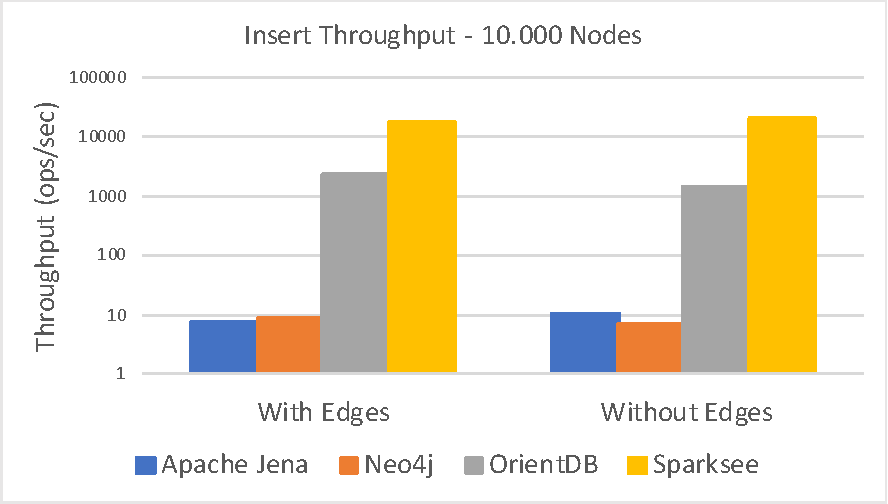
\includegraphics[width=.75\textwidth]{images/throughput/indexNoEdges10000Nodes}
  \caption{Comparison of insert throughput between using edges and not.}
  \label{fig:indexNoEdges10000Nodes}
\end{figure}

\subsubsection{Discussion}
\label{ch:evaluation:se:edgeDiscussion}
Figure~\ref{fig:indexNoEdges10000Nodes} shows an unexpected behaviour,
as the throughput of Neo4j and OrientDB is even higher when using edges,
whereas Apache Jena and Sparksee show a decrease in performance.
The largest differences can be seen for OrientDB and Sparksee,
but as their results point in two different directions we can only say,
that it depends on the database whether more edges affect the throughput negatively.

\section{Production Simulation}
\label{ch:evaluation:se:productionSimulation}
The workload results presented in this section will cover the production specific variables.
The first one is product complexity and the other one execution time.

\subsection{Product Complexity}
\label{ch:evaluation:se:productComplexity}
The product complexity describes,
how much the tree representing our data structure is widened at the three different levels shown in section~\ref{ch:design:se:dataStructure}.

The wider the data structure becomes the less edges we have per node and also we have more edges coming from one node to other nodes (one \texttt{Order} with multiple \texttt{Products} for example).
With that we can investigate the generalisation of graph structure,
to see whether other benchmark results from workloads with social network graphs can be used in an industrial application.

\subsubsection{Results}
In table~\ref{tab:structure} and figure~\ref{fig:structure} we see the impact different data structures have on the insert throughput.
"Simple" refers to the structure variables (x, y, z) set to (1, 1, 1),
"More Complex" represents (16, 32, 32) and "Most Complex" (64, 128, 128).

\begin{table}[h!]
  \begin{minipage}{\textwidth}
    \centering
    \begin{tabular}{ | l | l | l | l | }
      \hline
      Database & Simple & More Complex & Most Complex \\ \hline
      Apache Jena & 9,42 & 8,01 & 7,58 \\ \hline
      Neo4j & 11,44 & 11,64 & 8,5 \\ \hline
      OrientDB & 2606,5 & 2330,12 & 2118,38 \\ \hline
      Sparksee & 17345,38 & 17463,8 & 17576,06 \\ \hline
    \end{tabular}
  \end{minipage}
  \caption{Throughput in inserts/s, rounded to two decimal places, of the workload comparing different structure parameters.}
  \label{tab:structure}
\end{table}

\begin{figure}[h!]
  \centering
  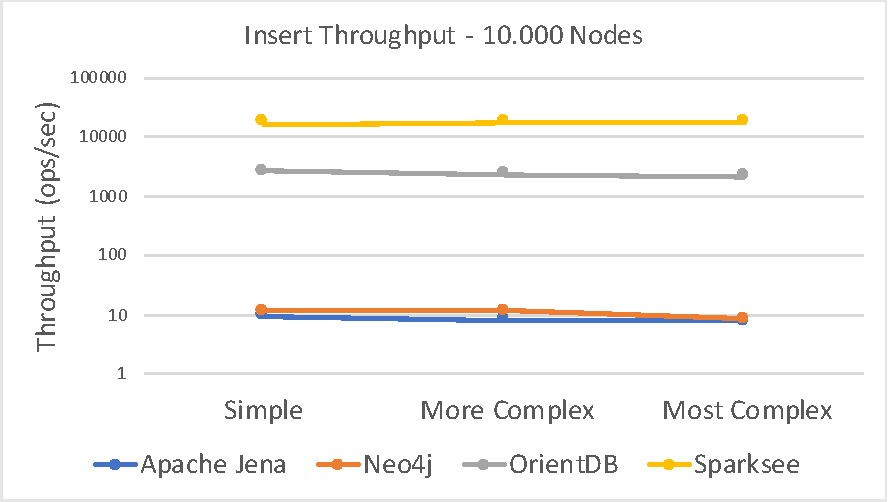
\includegraphics[width=.75\textwidth]{images/production/structure}
  \caption{Shows the difference in insert throughput over changing data structure.}
  \label{fig:structure}
\end{figure}

\subsubsection{Discussion}
As we see in figure~\ref{fig:structure} the structure of the data as we modelled it,
does affect the throughput of most databases, except Sparksee.
The throughput of the other three databases decreased with a more complex structure and a lower e/n ratio.

That fits into our findings from section~\ref{ch:evaluation:se:edgeDiscussion} where Neo4j and OrientDB showed a higher throughput with edges,
because the "Most Complex" workload has a lower e/n ratio.
Jena also seems to suffer from less edges per nodes,
what is contradictory to the experiment with no edges,
as Jena performed better without edges.

To draw a conclusion about the comparability with other related work using social network graphs,
which have a much higher e/n ratio,
we can at least say,
that depending on the database,
more edges can benefit the performance.

\subsection{Production Suitability}
\label{ch:evaluation:se:productionSuitability}
The production simulation will finally show,
whether the databases we chose are capable of storing the necessary amount of data in the specified time interval.

In the discussion of this section we will also investigate the throughput based on the previous workloads.

\subsubsection{Results}
Table~\ref{tab:singleSuitability} and figure~\ref{fig:singleSuitability} show how long OrientDB took,
to store three minutes of production data (1056833 nodes).
Sparksee is mentioned with a theoretical time,
since it only allowed us to store 1000000 elements.
We took the throughput during inserting these 1000000 elements and calculated the time it would need to complete the whole workload.

Only OrientDB and Sparksee were used in these workloads,
because Apache Jena and Neo4j would take much too long to insert that number of nodes.

\begin{table}[h!]
  \begin{minipage}{\textwidth}
    \centering
    \begin{tabular}{ | l | l | l | }
      \hline
      Database & Time (s) & Throughput (ops/sec) \\ \hline
      OrientDB & 263 & 8042,84 \\ \hline
      Sparksee & (134) & 15789,47 \\ \hline
    \end{tabular}
  \end{minipage}
  \caption{Time needed to execute three minutes of simulated production.
  The value in parentheses indicates a theoretical value,
  which was calculated with the throughput reached until the license ran out of size.}
  \label{tab:singleSuitability}
\end{table}

\begin{figure}[h!]
  \centering
  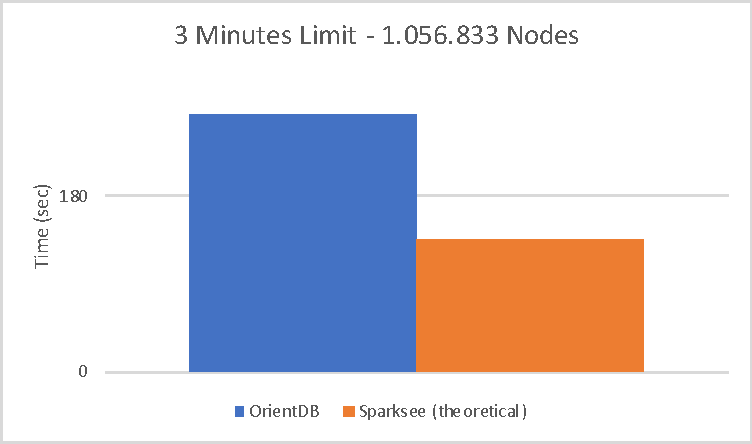
\includegraphics[width=.75\textwidth]{images/production/singleSuitability}
  \caption{Shows the execution time with a dataset that represents three minutes of production.}
  \label{fig:singleSuitability}
\end{figure}

\subsubsection{Discussion}
\label{ch:evaluation:se:suitabilityDiscussion}
We only executed three minutes of production simulation,
because the throughput of OrientDB doesn't grow anymore above 1000000 nodes (\ref{ch:evaluation:se:probingNodeCount}).
Therefore the one-hour workload wouldn't succeed either.

Figure~\ref{fig:singleSuitability} shows us,
that OrientDB didn't manage to store three minutes of production simulation in the specified time.

Sparksee could theoretically store that amount without exceeding the time limit.
Since the free license didn't allow for that amount of data,
we used the average until the limit was reached.
Of course,
it could be that the throughput of Sparksee drops with an increasing number of elements in the database,
but we couldn't investigate that.

The difference of this workload compared to the first workload we discussed in section~\ref{ch:evaluation:se:probingNodeCount} is the structure and the node size.
The results of~\ref{ch:evaluation:se:probingNodeSize} and~\ref{ch:evaluation:se:productComplexity} show,
that the structure has a slight impact on the throughput and the node size has no impact below $ 10KB $,
since we used $ 50B $ we can compare this to the throughput measured in ~\ref{ch:evaluation:se:probingNodeCount}.

By doing so we see that Sparksee,
theoretically,
exceeds our target throughput of $ 11743 \frac{inserts}{s} $.
OrientDB would have a throughput of $ 10112,36 \frac{inserts}{s} $ with a simple structure,
but since our "most complex" structure decreases OrientDBs throughput even more to only $ 8042,84 \frac{inserts}{s} $,
it would be even less suitable.

\section{Retrieving under load}
\label{ch:evaluation:se:retrievingUnderLoad}
This section will cover the results about retrieving data while the database is under load.
First,
we will take a look at how using an index is affecting the read and scan throughput.
Then we will compare the throughput of the different operations~(\ref{fig:operationReadScan}) and their impact on the insertion throughput~(\ref{fig:insertWithWithoutReadScan}).

\subsection{Results}
In tables~\ref{tab:readThroughput10000Nodes},
~\ref{tab:scanThroughput10000Nodes} and figures~\ref{fig:readThroughput10000Nodes},
~\ref{fig:scanThroughput10000Nodes} we see the throughput of read and scan operations while using an index and not.

\begin{table}[h!]
  \begin{minipage}{\textwidth}
    \centering
    \begin{tabular}{ | l | l | l | }
      \hline
      Database & Index & No Index \\ \hline
      Apache Jena & 47 & 49,11 \\ \hline
      Neo4j & 954,77 & 795,94 \\ \hline
      OrientDB & 8484,44 & 7816,22 \\ \hline
      Sparksee & 12411,84 & 989,3 \\ \hline
    \end{tabular}
  \end{minipage}
  \caption{Throughput in reads/s, rounded to two decimal places, of the workload using a mix of read and write operations.}
  \label{tab:readThroughput10000Nodes}
\end{table}

\begin{table}[h!]
  \begin{minipage}{\textwidth}
    \centering
    \begin{tabular}{ | l | l | l | }
      \hline
      Database & Index & No Index \\ \hline
      Apache Jena & 43,58 & 42,56 \\ \hline
      Neo4j & 574,17 & 495,58 \\ \hline
      OrientDB & 308,93 & 319,89 \\ \hline
      Sparksee & 174,28 & 135,41 \\ \hline
    \end{tabular}
  \end{minipage}
  \caption{Throughput in scans/s, rounded to two decimal places, of the workload using a mix of scan and write operations.}
  \label{tab:scanThroughput10000Nodes}
\end{table}

\begin{figure}[h!]
  \centering
  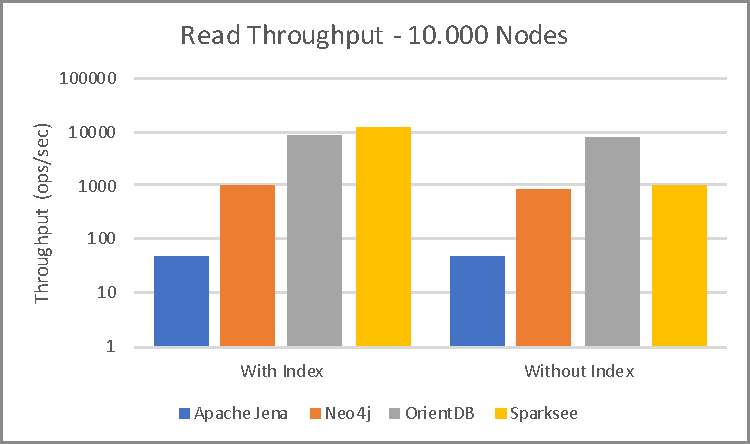
\includegraphics[width=.75\textwidth]{images/responsiveness/readThroughput10000Nodes}
  \caption{Shows the throughput of read operations with and without the use of an index.}
  \label{fig:readThroughput10000Nodes}
\end{figure}

\begin{figure}[h!]
  \centering
  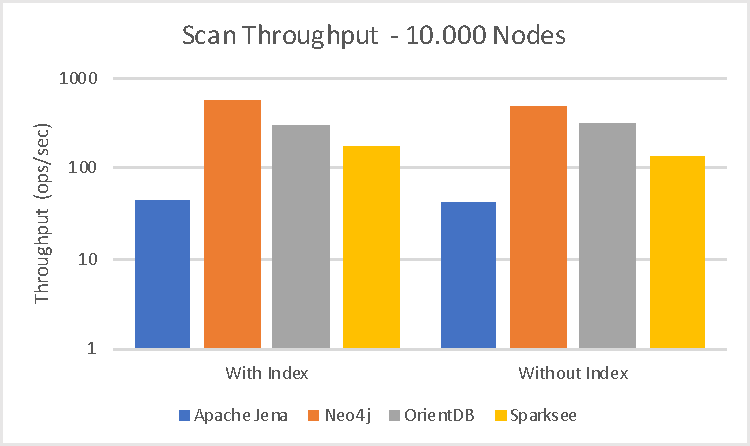
\includegraphics[width=.75\textwidth]{images/responsiveness/scanThroughput10000Nodes}
  \caption{Shows the throughput of scan operations with and without the use of an index.}
  \label{fig:scanThroughput10000Nodes}
\end{figure}

Figure~\ref{fig:operationReadScan} shows the throughput of the different operations.
In figure~\ref{fig:insertWithWithoutReadScan} and table~\ref{tab:insertWithWithoutReadScan} we see the impact of the read and scan operations on the insertion throughput.

\begin{table}[h!]
  \begin{minipage}{\textwidth}
    \centering
    \begin{tabular}{ | l | l | l | l | }
      \hline
      Database & Only Insert & With Read & With Scan \\ \hline
      Apache Jena & 9,42 & 6,35 & 7,15 \\ \hline
      Neo4j & 11,44 & 7,08 & 7,03 \\ \hline
      OrientDB & 2606,5 & 2180,7 & 1546,69 \\ \hline
      Sparksee & 17345,38 & 17162,63 & 17139,49 \\ \hline
    \end{tabular}
  \end{minipage}
  \caption{Throughput in inserts/s of insert operations, rounded to two decimal places, of the workloads using only insert, read or scan operations.}
  \label{tab:insertWithWithoutReadScan}
\end{table}

\begin{figure}[h!]
  \centering
  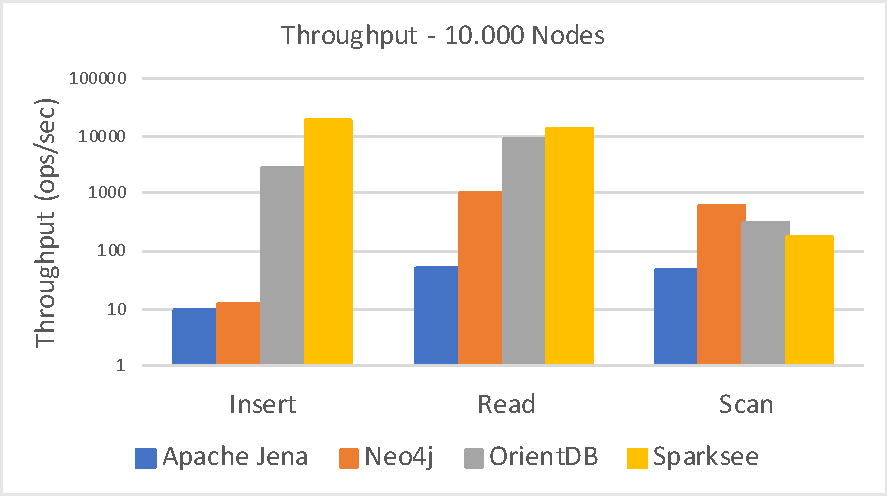
\includegraphics[width=.75\textwidth]{images/responsiveness/operationReadScan}
  \caption{Throughput in operations/s of the different operations.}
  \label{fig:operationReadScan}
\end{figure}

\begin{figure}[h!]
  \centering
  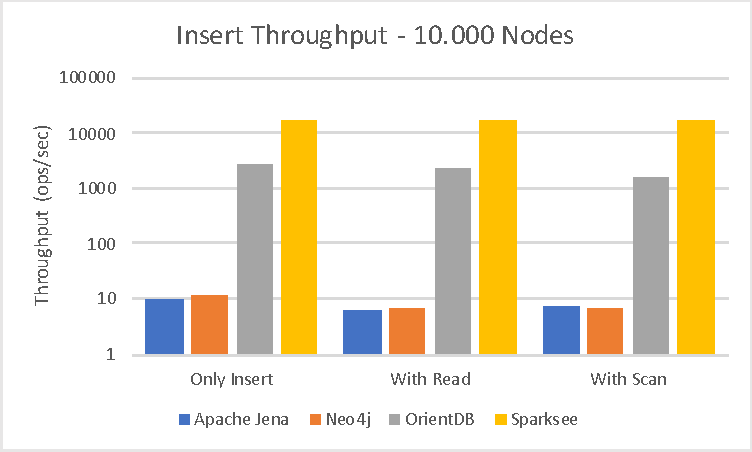
\includegraphics[width=.75\textwidth]{images/responsiveness/insertWithWithoutReadScan}
  \caption{Throughput in inserts/s without and with other operations.}
  \label{fig:insertWithWithoutReadScan}
\end{figure}

\subsection{Discussion}
First,
we will discuss the results regarding the use of an index and not.

For read operations,
figure~\ref{fig:readThroughput10000Nodes} shows,
that all databases benefit from using an index,
except Apache Jena which always uses an index and is only presented as reference.
Sparksee shows the biggest difference in throughput of read operations,
whereas the other databases only show a slight decrease in performance without an index.
That was what we would expect,
since an index really benefits these kinds of operations,
although we expected the increase with the use of an index to be higher for Neo4j and OrientDB.
The reason for that behaviour could be,
that the dataset size is too small to show a difference between using an index and not.

Similar results can be seen for the scan operations,
shown in figure~\ref{fig:scanThroughput10000Nodes}.
The absence of an index doesn't show much effect here either.
That could be the case,
because scan operations only use one read operations for the start node and then traverse the graph,
which isn't affected by the index.

The comparison of the different operations,
shown in figure~\ref{fig:operationReadScan}, shows us where the strengths and weaknesses are of the different databases.\\
Apache Jena and Neo4j are the slowest when it comes to inserting nodes,
but they are much faster in retrieving nodes,
with Neo4j even being the fastest of all for in graph traversal.\\
This also explains why Neo4j and OrientDB have a higher throughput when using edges,
because they can look up the edges much faster than they can insert a node.
That also concludes,
that the insertion part of creating an edge is cheap compared to inserting a node.

OrientDB and Sparksee seem to be a good choice when inserting and reading is the main concern of the application.

When we compare the results of Apache Jena from its read performance to its scan performance,
we see almost no difference in performance,
which means it is even faster than Neo4j in graph traversal,
but it is limited by the relatively slow read operation at the beginning of the scan operation.

The last figure~\ref{fig:insertWithWithoutReadScan} shows us,
that using other operations on the database does effect insert throughput,
except for Sparksee.
It seems to stay stable in its throughput even when other operations are being used.

Jena and Neo4j are low in throughput anyways,
but they still suffer from other operations being executed regularly.
OrientDB has a slightly worse throughput when using read operations and even worse with scan operations.
That is important to know for an industrial application,
where read and scan operations are executed more or less regularly,
because the database would decrease in its general performance.

\section{Related Work and Generalisability}
\label{ch:evaluation:se:relatedWorkAndGeneralisability}
In this section we will compare our results with the findings of our related work as it's suitable.
Our main goal is to investigate whether the difference in structure and e/n ratio has an impact on performance.
If that isn't the case we can assume,
that benchmark results from research on social network graph can be used to evaluate the performance of a graph database in an industrial environment.\\
The key point we will investigate is how the number of edges in relation to the number of nodes affects the throughput performance of the databases.
In social network graphs this number is quite high at around $ 8 $~\cite[41]{TaoShen} to $ 22 $~\cite{Dayarathna2012},
whereas our graph structure contains an e/n ratio of $ 1.3 $ to $ \sim1 $ (depending on the variables x, y and z (higher variable values lead to a ratio closer to 1) or $ 0 $ when we compare to the workload without edges.

By comparing our finding with the ones from Dominguez-Sal et al.~\cite{TaoShen},
which can be seen in figure~\ref{fig:throughputShen},
we see,
that all databases performed much better than in our experiment.
The throughput of Neo4j and Jena is well above $ 100 \frac{inserts}{s} $ and Sparksee also reaches a higher throughput with $ 29770 \frac{inserts}{s} $.\\
Our findings would suggest,
that their performance for Sparksee and Jena should be lower than ours and Neo4j would perform better,
but since all databases perform better something else has to be different in their case.\\
The better performance could be the results of a lack of information stored in the nodes,
as the paper only mentions weights on the inserted edges we cannot surely tell whether that is the case.

With this comparison we would conclude,
that graph databases perform worse in an industrial environment,
where graphs that have a lower e/n ratio compared to a social network graph.\\
Therefore,
the results of other benchmarks executed on graph databases with social network graph cannot be used to determine the throughput in an industrial application,
as we can't tell how much throughput is sacrificed by storing any information in the nodes.
We investigated the impact of different node sizes,
but to measure the throughput with absolutely no information in the nodes a different implementation would be required which doesn't use the methods to store information in the nodes.

\begin{figure}[!h]
  \centering
  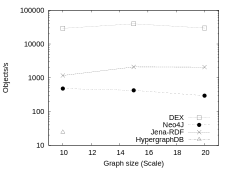
\includegraphics[width=.8\textwidth]{images/benchmarks/ShenResultsInsert}
  \caption{Throughput results of Dominguez-Sal et al.~\cite{TaoShen}.}
  \label{fig:throughputShen}
\end{figure}

The research of Dayarathna et al.~\cite{Dayarathna2012} used a e/n ratio of 22 with a node count of only 1024.
Comparing their results shown in figure~\ref{fig:throughputXGDBench} with our results from figure~\ref{fig:withIndexThroughput} leads to the conclusion,
that the databases perform better with an industrial graph structure and less edges.\\
But by looking closer at the data and our findings from the workload using no edges in section~\ref{ch:evaluation:se:edgeDiscussion} we would expect that the results would be better for OrientDB and Neo4j since they both performed better with more edges.\\
Overall this comparison leads to the conclusion,
that graph databases perform better with industrial data structures.

\begin{figure}[!h]
  \centering
  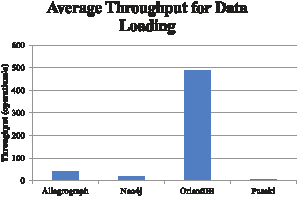
\includegraphics[width=\textwidth]{images/benchmarks/XGDBenchResultsInsert}
  \caption{Throughput results of the XGDBench Benchmark~\cite{Dayarathna2012}.}
  \label{fig:throughputXGDBench}
\end{figure}

If we look at our own findings in figure~\ref{fig:indexNoEdges10000Nodes} we can come to the following conclusion.\\
The better the read performance is compared to the insert performance, the better the graph database performs with more edges.
That would correlate with Dominguez-Sal et al.~\cite{TaoShen},
as they have a higher e/n ratio and better throughput.

To generalise our finding based on the comparison with other research in this field,
no clear conclusion can be drawn as the results diverge.\\
When taking into account our findings about the dependency between insert and read operations,
we can say that other benchmark results can be used to evaluate the suitability of a database for the industrial environment when the insert and read throughputs are listed.
